\documentclass[man]{apa2}

\usepackage{pdfsync}
\usepackage{apacite}
\usepackage{amsmath}
\usepackage{graphicx}
\usepackage{topcapt}
\usepackage{color}
\usepackage{inputenc} 

\title{Social information, referential uncertainty, and multiple alternatives tracking in cross-situational word-learning

(Submitted for the First-Year Project)}
\author{Kyle MacDonald}
\affiliation{Department of Psychology, Stanford University}

\vspace{3.0ex}

\shorttitle{Social cues and cross-situational word-learning}
\rightheader{SOCIAL INFORMATION AND CROSS-SITUATIONAL LEARNING}
\leftheader{Kyle MacDonald}

\begin{document}
\maketitle


%%%%%%%%% ABSTRACT  %%%%%%%%% 
\section{Abstract}

Word learning proceeds despite the potential for referential uncertainty: within a naming context, a new word could refer to many possible objects, properties of those objects, or even nothing at all. Both social cues and word-object co-occurrence statistics can reduce this uncertainty. But how do learners integrate these two information sources? In a large-scale experiment, we show that the presence of social cues during labeling modulates learners' tracking of cross-situational statistics: without social cues, learners are more likely to track multiple word-object links. Further, I present a computational model that takes a first-step in formalizing how social information influences cross-situational word learning. Together, the data and model suggest that there is a rational tradeoff between reducing uncertainty and the type of representations that learners store.  

\newpage


%%%%%%%%% INTRO %%%%%%%%% 
\section{Introduction}
Language is a powerful tool that allows us to rapidly learn from others and building a large early vocabulary creates the foundation for later language and academic success \cite{hart1995meaningful, qian2002investigating}. But, to learn the meaning of a new word \footnote{Here I focus on the task of mapping concrete nouns to objects, assuming that the child has solved other requisite inferential problems, e.g., word segmentation.}, children must solve the core problem of referential uncertainty \cite{quine19600}: that the range of potential referents for a new word is largely unconstrained. So how do learners reduce this uncertainty?

Social-pragmatic theories argue that the social context of word learning simplifies the word-object mapping problem \cite{bloom2002children, tomasello2009constructing}. Associative approaches suggest that the rich structure of language allows children to learn new words by tracking word-object co-occurrences over time (i.e., cross-situational learning) \cite{smith2008infants}. Importantly, these two information sources function at different timescales, with social cues reducing uncertainty during an individual naming event and cross-situational statistics reducing uncertainty across multiple naming events. Moreover, within the cross-situational learning literature, there is considerable debate about the underlying mechanisms that support this type of learning: do learners track information about multiple referents or store a single candidate referent?

In this paper, we explore how learners integrate social and cross-situational information and how this interaction modulates the type of representation that learners store. First, I will review evidence in support of children's ability to use both social cues and cross-situational statistics to reduce uncertainty during word learning. Then I will present the debate over the type of representations that learners store during cross-situational word-learning. Finally, I will present data from a large-scale experiment and a computational model that together show a tradeoff between the presence of social information and the type of cross-situational information that learners store.

%%%%%%%%% SOCIAL CUES - IN-THE-MOMENT  %%%%%%%%% 

\section{Reducing referential uncertainty}

\subsubsection{Social cues}

Social cues, such as eye gaze and pointing, can facilitate word-learning by reducing the number of potential referents for a new word.  Consider a labeling context in which the child is surrounded by new toys and hears a speaker say a novel word. Without any additional cues to reference, mapping that word to one of the objects would be difficult. But, if the speaker is holding only one of the toys, then the mapping challenge is simplified because the child can make a stronger inference about the speaker's referential intent. Social Pragmatic theories emphasize the importance of this type of uncertainty reduction for word-learning \cite{bloom2002children, tomasello2009constructing}.

Experimental work shows that children as young as 16 months are sophisticated intention-readers, preferring to map novel words to objects that are the target of a speaker's gaze during labeling, not their own\cite{baldwin1993infants,baldwin2001links}. More recent research suggests that labeling contexts accompanied with rich social cues provide the child with clear visual access to objects during naming, creating an ideal word-learning situation \cite{yu2012embodied}. Further, correlational data show strong links between early intention-reading skills (e.g., gaze following) and later vocabulary growth in typically-developing children \cite{brooks2008infant} and children diagnosed with autism \cite{mundy1990longitudinal}. 

But, not all of children's learning experiences occur in rich social contexts. 





\section{Single vs. multiple referent tracking}





In the second version, children were familiarized with four objects hidden at four different locations, one of which was a particularly salient toy barn. Once the child had linked each object to its hiding place, an adult announced her intention to "find the gazzer." She then went to the hiding location of the toy barn, but it was locked and she frowned upon not being able to open it. She then continued her search to one of the other hiding locations, saying "Let's see what else we can find," and pulled out a distractor object while smiling. Interestingly, 18- and 24-month old children mapped the novel word "gazzer" to the toy barn, even though they had not seen the barn after hearing the word and the adult had smiled at a distractor object. 

The common thread across all of these studies is that children could not have relied on saliency and co-occurrence information to learn the novel word meanings because the words and objects did not occur close in time and the distractor objects were often more salient. In addition, children were able to use social cues flexibly to determine referential intent: In the first finding game, a smile indicated referential intent, but in the second game, a frown was the relevant cue. Thus, even at 18 months, children are able to infer adults' referential intent and use this information to guide their word-learning in non-ostensive contexts.

\subsubsection{Joint Attention}

Social Pragmatic theories also emphasize the importance of episodes of joint attention for early word-learning. These episodes involve a caregiver and child attending to an object and understanding that the other participant is also attending to that same object \cite{carpenter1995joint, tomasello1983joint}. These contexts are highly structured, repetitive, and limited to a handful of referential intentions, thus simplifying the child's inference. Experimental data show that joint attention facilitates language acquisition \cite{brooks2008infant,farrar1993event}. More recent research suggests that joint attention episodes, in addition to making referential intent clear, provide the child with clear visual access to objects during naming, creating an ideal word-learning situation \cite{yu2012embodied}. Correlational data also show strong links between early joint attention skills (e.g. pointing and responding to parental bids for attention) and later vocabulary growth in typically-developing \cite{tomasello1986joint, carpenter1998social,farrant2012early} and children diagnosed with autism \cite{mundy1990longitudinal}.

Additional evidence in support of the importance of rich social interactions for language acquisition comes from recent research investigating the relationship between children's early language environments and language skills. \citeA{weisleder2013talking} measured children's language processing skills, vocabulary, and recorded parent-infant interactions at home using a digital audio recorder that could capture up to 16 hours of speech. These audio recordings were coded for the amount of speech directed to the child and the amount of speech overhead by the child. Importantly, infants who experienced more child-directed speech, but \emph{not overhead speech}, were more efficient in processing language and had larger vocabularies. 

Together, there is sufficient evidence that rich, social interactions are high in information value and facilitate early word-learning. However, these episodes make up only a portion of the word-learning contexts that young children experience \cite{frank2013social} and children can learn language without experiencing much direct social interaction with adults \cite{shneidman2012language}. So how might children, in the absence of rich, social information, learn the meanings of words? 

%%%%%%%%% XSL OVER TIME  %%%%%%%%% 

\section{Associative word-learning}

Associative accounts of word-learning highlight children's powerful statistical learning mechanisms, which track the regularity present in natural language, allowing the learner to map words to objects over time. Researchers in support of this proposal point out that children in early stages of word-learning, before 18 months of age, often have difficulty disambiguating referential intent and infants at much younger ages (8 months) show sensitivity to statistical information in both the auditory \cite{saffran1996statistical} and visual \cite{fiser2002statistical} domains. In this account, word-learning is best explained by domain-general pattern-finding abilities, attention, and memory and words are often mapped to the most salient object in the visual scene.

Empirical data show that in the absence of social cues to word meaning, adults and children are able to rapidly learn words by tracking the co-occurrence of labels and objects across multiple, ambiguous exposures \cite{smith2008infants,vouloumanos2008fine}. For example, \citeA{smith2008infants} taught children three novel words simply by repeating consistent novel word-object pairings across 10 ambiguous exposure trials. Each exposure consisted of two novel objects and one novel word, with no social cues to reference. Importantly, there was no way for children to infer the correct meaning of the novel word on any one trial, but over time, they accumulated statistical information that led them to make the correct mapping. These results provide strong evidence of children's ability to track the co-occurence statistics of words and objects in the service of word-learning. 

In summary, a substantive body of research supports both the Social-Pragmatic and Associative accounts of early word-learning. However, word-learning requires solving both social-cognitive and mapping challenges simultaneously. Thus, it is likely that children use multiple skills and a variety of information sources to learn words, both social and data-driven. In the next section, I will review experimental and computational work that attempts to take this complexity into account and integrate Social-Pragmatic and Associative accounts. 

%%%%%%%%% INTEGRATIVE APPROACH  %%%%%%%%% 

\section{Integrating Social and Associative Learning}

Integrated accounts of early word-learning emphasize the impact of multiple factors on children's ability to learn new words. For example, \citeA{hollich2000breaking} propose an Emergentist Coalitional Model in which they suggest that children take advantage of a "coalition" of cues - social, associative, and linguistic - to learn words. Importantly, these cues are always available to the learner and what changes is how children use each cue. Empirical work provides support for the idea that children do use different sources of information to learn words and the use of specific types of cues changes with development. Using a preferential looking task, \citeA{hollich2000breaking} asked children aged 10, 12, 19, and 24 months to learn novel words for objects, and pitted social and perceptual cues against each other to test the usefulness of each information source for making the correct object-word mapping at each age. Interestingly, the youngest children ignored the social cue of experimenter eye gaze (i.e., child-guided joint attention), preferring to map the novel word to the more visually salient object (in line with predictions made by the Associative account);  however, the older children (20 months and older) preferred to map novel words to the object that the adult labeled. 

Recent computational models attempt to formalize how social and statistical cues can be integrated to facilitate word-learning \cite{yu2007unified,frank2009using}. These models, however, treat social information in fundamentally different ways. In \citeA{yu2007unified} Unified Model, social information, such as eye gaze or prosody, is characterized as a "spotlight" that directs the child's attention to objects in the visual scene. In this account, social cues are considered, but intention reading is secondary to attention and saliency. Put another way, social cue simply adds weights to the words and objects that allow statistical learning to operate more effectively. 

In contrast, \cite{frank2009using} propose an \emph{Intentional} model that characterizes social information as providing evidence of a speaker's referential intent, which in turn facilitates word-learning. This model assumes that the relationship between words and objects is mediated by the speaker's goals to refer to some object. By making inferences about a speaker's referential intent, the model is able to simultaneously solve both the social-cognitive and mapping inference problems inherent to word-learning. In addition, Frank and colleagues were able to capture many seminal findings in the early word-learning literature, including cross-situational learning and the use of inferred intentions to disambiguate reference.

In the final section, I propose a new study that follows this line of empirical work and modeling\cite{johnson2012exploiting,frank2009using,yu2007unified,hollich2000breaking} and explores the interaction between social and statistical learning.

%%%%%%%%% CURRENT WORK  %%%%%%%%% 

\section{Current Work}

Several studies show that in the absence of social cues to word meaning, adults and children are able to rapidly learn words by tracking the co-occurrence of labels and objects across exposures (i.e. cross-situational learning) \cite{smith2008infants,vouloumanos2008fine}. However, some researchers question the psychological plausibility of these gradualist accounts, suggesting that children's rapid word learning is better described by a single hypothesis tracking mechanism \cite{trueswell2013propose,medina2011words}. 

Recent experimental work shows that both adults and children can track and recall 
multiple referents (Yurovsky & Frank, in prep). In Yurovsky and Frank's task, participants saw a set of novel objects and heard a novel word (e.g. Grink), and were asked to make a guess about the "correct"\footnote{There was actually no "correct" answer on exposure trials; rather these trials gave participants evidence about potential word-object mappings and allowed them to form an initial hypothesis.} word-object mapping. In subsequent test trials, participants heard the novel word again, this time paired with another set of novel objects. Critically, one of the objects in the set was either the participant's initial hypothesis (Same trials) or one of the objects that was \emph{not} the initial hypothesis (Switch trials). On Switch trials, adults reliably selected the object that was not their initial hypothesis, even when there were eight objects in the initial exposure set, providing strong evidence that learners track multiple referents when learning new words. 

However, this task did not include any of the rich, social cues that typically accompany real world 
word-learning. So it is still an open question as to how social information interacts with learners' 
demonstrated ability to track multiple referents. Perhaps the presence of additional evidence about 
a speaker's referential intent strengthens the learner's initial hypothesis, reducing the need to track 
alternative hypotheses. Or social information could strengthen the initial hypothesis 
without reducing multiple referent tracking. The proposed study asks if the presence of social information changes how learners track multiple referents when learning new words?

The answer to this question will increase our understanding of how social information interacts with statistical learning mechanisms with the overarching goal of clarifying the unique contribution of each information source to children's early word learning. 

%%%%%%%%% EXPERIMENT  %%%%%%%%% 


\section{Experiment}

\subsection{Participants}

This experiment was posted to Amazon Mechanical Turk as a set of
Human Intelligence Tasks (HITs) to be completed only by participants with US IP
addresses that paid 30 cents each (for a detailed comparison of laboratory and Mechanical
Turk studies see \citeNP{crump2013evaluating}). 30 HITs were posted for each
condition (Social, Non-social) for total of 60 paid HITs. If a participant
completed the experiment more than once, he or she was paid each time but only data
from the first HITs completion was included in the final data set. In
addition, data was excluded from the final sample if participants did not give correct
answers for familiar trials (excluded 1 HIT).

\subsection{Stimuli}

Stimuli for the experiment consisted of black and white pictures of familiar
and novel objects, a schematic drawing of a human interlocutor, and audio recordings of familiar and novel words. Pictures of 32 familiar objects spanning a range of categories (e.g. squirrel, truck, tomato, sweater) were drawn from the set constructed by \citeA{snodgrass1980standardized}. Pictures of distinct but
difficult to name objects were drawn from the set of 140 first used in \citeA{kanwisher1997locus}. For ease of viewing on participants' monitors, pixel values for all pictures were inverted so that they appeared as white outlines on black backgrounds (see Figure 1). Familiar words consisted of the labels for the familiar objects as produced by AT&T Natural VoicesTM (voice: Crystal). Novel words were 1-3 syllable pseudowords obeying the rules of English phonotactics produced using the same speech synthesizer.
%
\begin{figure}
	\centering
	\fbox{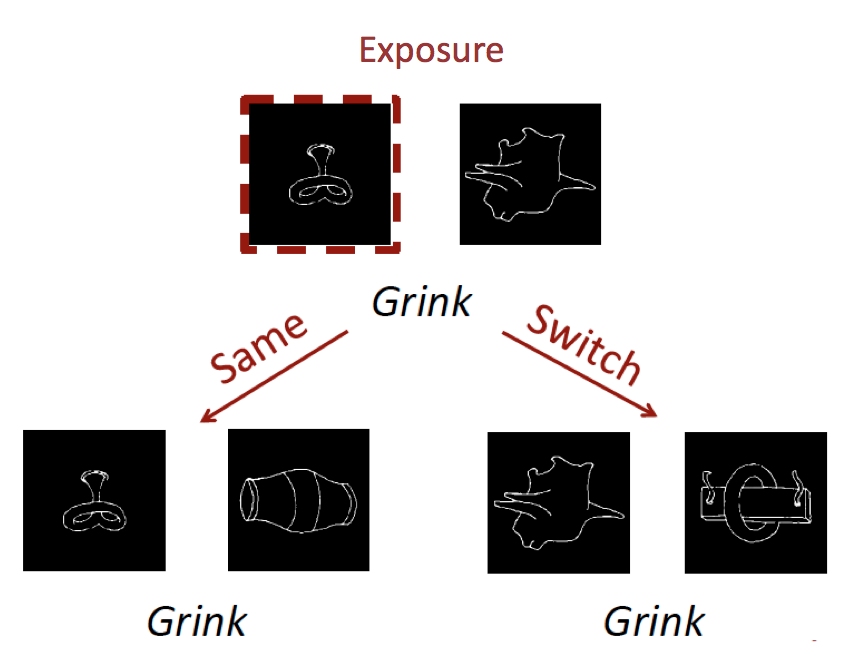
\includegraphics[scale=0.22]{stimuli2.png}}
	\caption{A schematic of the trials that participants saw in the experiment. On Exposure trials, participants saw four novel objects and heard a novel word. Participants were asked to guess it's correct referent. After the Exposure trial, participants either saw a Same or a Switch trial. On Same trials, the set of four referents contained the participant's previous hypothesis. On Switch trials, the set of referents contained one of the objects that the participants had \emph{not} hypothesized.}
\end{figure}

A schematic drawing of a human interlocutor was chosen for ease of manipulating the direction of eye gaze, the social cue of interest in this study. Five images were created using Adobe Photoshop with the following directions of eye gaze: far left, close left, close right, far right, and eyes center. Because this task was performed over the internet and participants' screen sizes might be small, it was important to make the eye gaze cue clear.
%
\begin{figure}
	\centering
	\fbox{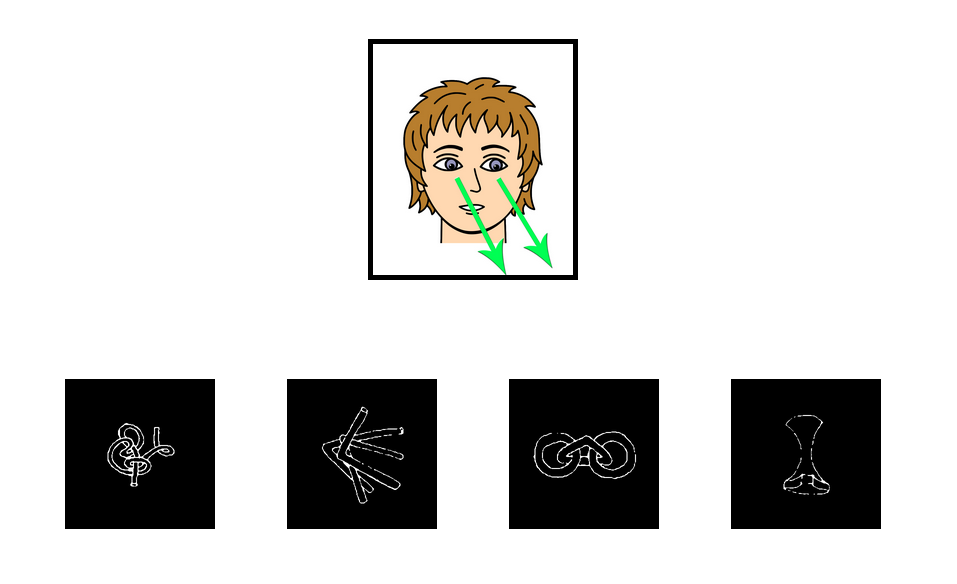
\includegraphics[scale=0.2]{stimuli1.png}}
	\caption{Exposure trials in the Social condition. In the Nonsocial condition, the interlocutor looked straight ahead during exposure. During test trials, the interlocutor looked straight ahead.}
\end{figure}
%
\subsection{Design and Procedure}
Participants were exposed to a series of trials in which they heard an interlocutor say a novel word, saw
four novel objects, and were asked to indicate their guess as to which object was the
referent of the word. After a written explanation of this procedure, participants were given
four practice trials to introduce them to the task. On each of these trials, they heard the interlocutor say a
Familiar word while looking at a line drawing of that object among a set of other familiar objects.
On the first two trials, participants were asked to find the squirrel, and the correct answer
was in the same position on each trial. On the next two trials, participants were asked to
find the tomato, and the correct answer switched positions from the first to the second
trial (in order to ensure that participants understood that the on-screen position was not
an informative cue to the correct target). These trials also served to screen for participants
who did not have their audio enabled or who were not attending to the task.

After these Familiarization trials, participants were informed that they would now hear
novel words, and see novel objects, and that they should continue selecting the correct
referent for each word. Participants each heard eight novel words twice. Participants saw four referents
on each trial, and the two trials for each word occurred back-to-back. Four of these
follow-up trials were Same trials in which the referent that participants selected on the exposure trial appeared again amongst the set of objects. The other four were
Switch trials in which one of the referents in the set was selected randomly from the objects
a participant did not select on the previous Exposure trial. All other referents were
completely novel on each trial. Critically, on Exposure trials the interlocutor's eye gaze was directed and thus informative, but on Same/Switch trials her eye gaze was undirected and thus uninformative. 

Participants were randomly assigned to one of two conditions: Social or Nonsocial. In the Social condition, eye gaze was informative on exposure trials. In the Nonsocial condition, eye gaze was uninformative throughout the task, i.e. the speaker always looked straight ahead. 

Because participants performed this task over the internet, it was important to
indicate to them that their click had been registered. Thus, a red dashed box appeared
around the object they selected for 1 second after their click was received. This box
appeared around the selected object whether or not it was the "correct" referent.




%%%%%%%%% STUDY - RESULTS  %%%%%%%%% 



%%%%%%%%% MODEL  %%%%%%%%% 


\section{Model}

First, I begin by describing the computational model developed by \citeA{frank2009using} and extended by Yurovsky and Frank (in prep). Then, I will discuss how I modified the model's parameters in order to generate predictions about the effect of social cues to reference on cross-situational learning. 

In \citeauthor{frank2009using}'s model, the word-learning problem is defined by a set of variables and probabilistic dependencies that link these variables. The learner observes a set of situations \emph{S}, which consist of two observed variables - objects (\emph{O}) and words (\emph{W}) - and one hidden variable: the speaker's intention (\emph{I}), with the goal of inferring the most probable lexicon of word-object mappings (\emph{L}) given the set of observed situations. Formally, the task of learning the correct lexicon can be defined as a problem of Bayesian inference: 
%
\begin{equation}
\label{1}
P(L|S) \propto P(S|L)P(L)
\end{equation}
%
The likelihood term ($P(S|L)$) captures the learner's assumptions about the task. Each situation (\emph{S}) includes a word, a set of objects, and the speaker's referential intention (\emph{I}). Thus, $P(S|L)$ can be expanded and the probability of the lexicon can be given as: 
%
\begin{equation}
\label{2}
P(L|S) \propto \prod\limits_{s \in S}  P(W_s, I_s, O_s|L)P(L)
\end{equation}
%
Because referential intention mediates the relationship between words and objects, the likelihood term can be rewritten as:
%
\begin{equation}
\label{3}
P(L|S) \propto \prod\limits_{s \in S}  P(W_s|I_s, L)P(I_s|O_s)P(L)
\end{equation}
%
The prior probability of a lexicon is defined as: $P(L_o) \propto \frac{1}{|L_o|}$, which is a parsimony prior that favors lexicons with fewer words referring to the same object. 

Thus far, I have described the computational problem for the Bayesian word learner outlined by \citeNP{frank2009using}. Yurovsky and Frank then extended this computational level description to include cognitive constraints (memory and attention), allowing them to provide an algorithmic-level account of their data. Memory was modeled as a power function that took into account the interval between successive exposures to a word. The $\gamma$ parameter scaled to the strength of the initial encoding and the $\lambda$ parameter defined the rate of decay.
%
\begin{equation}
\label{4}
M(L_o) =  \gamma L_ot^{-\lambda}
\end{equation}
%

Attention was defined in terms of the learner's belief about $P(I|O)$: the probability of the speaker's intention to refer to each object in the set. The $\sigma$ parameter captures the amount of probability mass that the learner  places on each referent during the initial exposure. The strength of the learner's belief about $P(I|O)$ in turn directly influences the strength of initial encoding. At $\sigma = 1$, the learner is placing all of the probability mass on one word-object mapping (i.e. a single hypothesis tracking strategy). At $\sigma = \frac{1}{|O|}$, the learner is distributing the probability mass across all possible word-object mappings equally (i.e. a parallel statistical accumulator strategy). 

Figure 1 shows model predictions for four different levels of belief about referential intent (i.e. four different values for $\sigma$). The first two models are from Yurovsky and Frank (in prep). The Parallel Accumulator model, $\sigma = (\frac{1}{|\sigma|})$, predicts indistinguishable performance on Same and Switch trials because the learner is allocating belief evenly across referents. The No Social Integrated model predicts strong performance on Same trials and above chance performance on Switch trials because it allocates a chunk of probability to a single hypothesis and distributes the rest to the other referents. This model was the best fit for human behavior on their cross-situational learning task, explaining 98\% of the variance in the data. 

However, these two models did not include the rich social cues to reference that are available to the word learner. Perhaps more evidence about referential intent will cause the learner to place more belief on the object that is the target of the referential act. To formalize this intuition, I modified the $\sigma$ parameter in Frank and Yurovsky's model to generate predictions about human performance on a social, cross-situational learning task (see Figure 1). The Weak Social model treats social information as additional evidence about reference, and increases the allocation of belief to a single hypothesis, $\sigma = 0.75$. It predicts an improvement on Same trials and a decrease in performance on Switch trials. However, the learner still tracks multiple referents and does not place \emph{all} belief on a single hypothesis. In contrast, the Strong Social model ($\sigma = 1$) predicts that learners will not track multiple referents because all of their probability mass is allocated entirely to the target of the speaker's referential intent, similar to the single-hypothesis tracking strategy suggested by Trueswell and colleagues. 



%%%%%%%%% DISCUSSION  %%%%%%%%% 




\bibliographystyle{plain}
\bibliography{fyp_p}

\end{document}
